\documentclass{article}
\usepackage[utf8]{inputenc}
\usepackage{graphicx}

\title{Bohr's Theory}
\author{Julia Abibe}
\date{January 28, 2016}

\begin{document}

\maketitle

\section{Theory of the electron}
It consists of four principles:

1) Electrons assume only certain orbits around the nucleus. These orbits are stable and called "stationary" orbits.

2) Each orbit has an energy associated with it. For example the orbit closest to the nucleus has an energy E1, the next closest E2 and so on.

3) Light is emitted when an electron jumps from a higher orbit to a lower orbit and absorbed when it jumps from a lower to higher orbit.

4) The energy and frequency of light emitted or absorbed is given by the difference between the two orbit energies, ex:

$$E(light)=Ef-Ei$$
$$n= \frac{E(light)}{h}$$
$$h= 6.627 \times 10^{-34} J$$

\begin{figure}[h]
\begin{center}
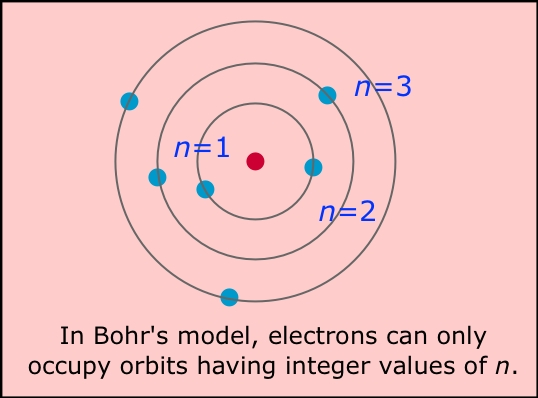
\includegraphics[width=0.4\textwidth]{bohr1.jpg} % Include the image placeholder.png
\caption{Bohr's Model}
\end{center}
\end{figure}

\section{Observed spectra of emitted light of excited hydrogen}

Each spectral line represents an energy difference between two possible states of the atom. Each of these states corresponds to the electron in the hydrogen atom being in an "orbit" whose radius increases with the quantum number n. The lowest allowed value of n is 1; because the electron is as close to the nucleus as it can get, the energy of the system has its minimum (most negative) value. This is the most stable state of the hydrogen atom, and is called the ground state.

\begin{figure}[h]
\begin{center}
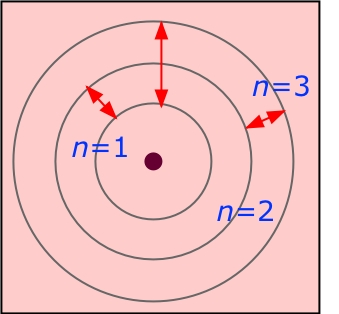
\includegraphics[width=0.4\textwidth]{BohrModel-2} % Include the image placeholder.png
\caption{Bohr Model}
\end{center}
\end{figure}


If a hydrogen atom absorbs radiation whose energy corresponds to the difference between that of n=1 and some higher value of n, the atom is said to be in an excited state. Excited states are unstable and quickly decay to the ground state. For example, if the electron is initially promoted to the n=3 state, it can decay either to the ground state or to the n=2 state, which then decays to n=1.

If, instead, enough energy is supplied to the atom to completely remove the electron, we end up with a hydrogen ion and an electron. When these two particles recombine (H+ + e– → H), the electron can initially find itself in a state corresponding to any value of n, leading to the emission of many lines.

The lines of the hydrogen spectrum can be organized into different series according to the value of n at which the emission terminates. The lines in each series crowd together as they converge toward the series limit which corresponds to ionization of the atom and is observed as the beginning of the continuum emission.

\begin{figure}[h]
\begin{center}
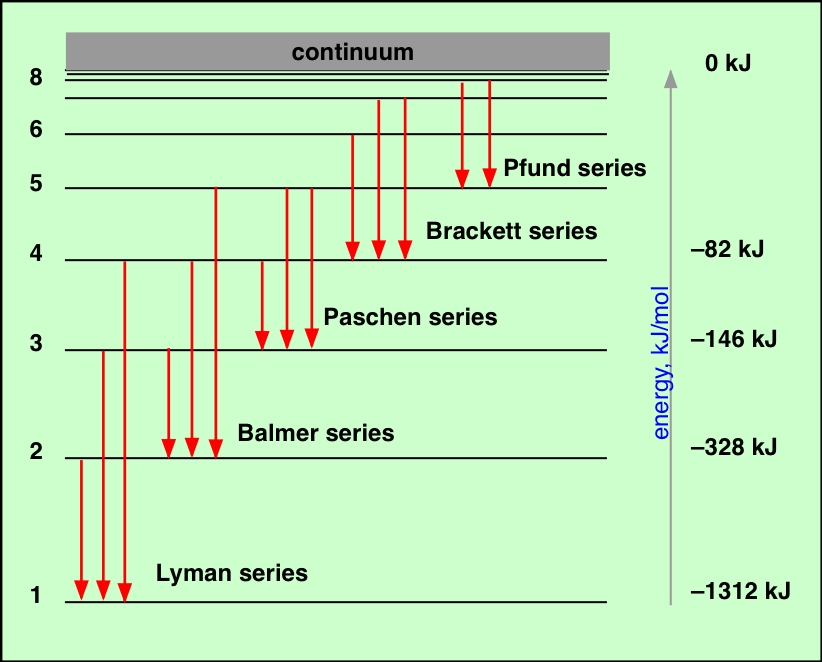
\includegraphics[width=0.4\textwidth]{spectral} % Include the image placeholder.png
\caption{Spectral Series}
\end{center}
\end{figure}


Although an infinite number of n-values are possible, the number of observable lines is limited by our ability to resolve them as they converge into the continuum; this number is around a thousand.

\section{First hydrogen spectra - Lyman series}

Discovered the spectral lines from 1906–1914. All the wavelengths in the Lyman series are in the ultraviolet band.

\begin{figure}[h]
\begin{center}
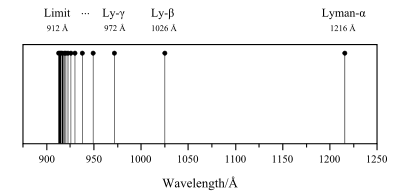
\includegraphics[width=0.4\textwidth]{Lyman} % Include the image placeholder.png
\caption{Lyman series}
\end{center}
\end{figure}

\begin{figure}[h]
\begin{center}
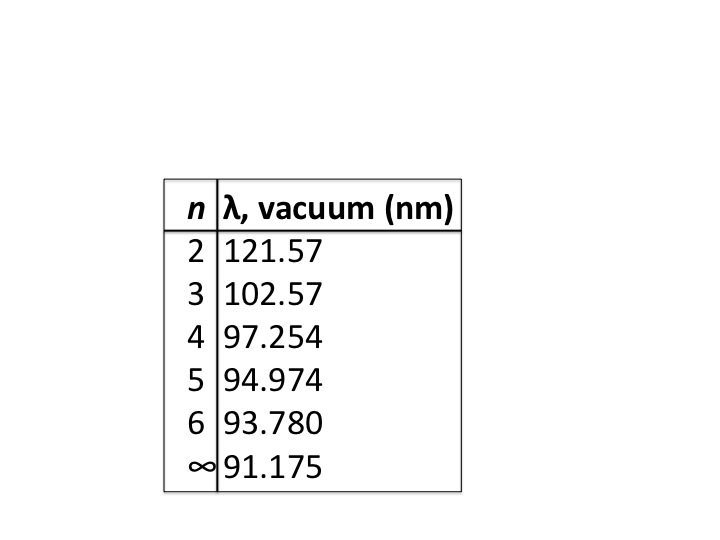
\includegraphics[width=0.4\textwidth]{lymantable} % Include the image placeholder.png
\caption{Table}
\end{center}
\end{figure}


\section{Second hydrogen spectra - Balmer series}

Balmer lines are historically referred to as "H-alpha", "H-beta", "H-gamma" and so on, where H is the element hydrogen.[8] Four of the Balmer lines are in the technically "visible" part of the spectrum, with wavelengths longer than 400 nm and shorter than 700 nm. Parts of the Balmer series can be seen in the solar spectrum. H-alpha is an important line used in astronomy to detect the presence of hydrogen.

\begin{figure}[h]
\begin{center}
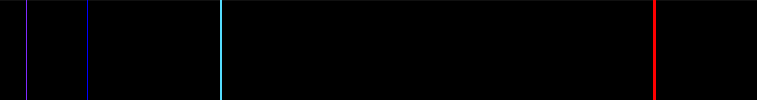
\includegraphics[width=0.4\textwidth]{balmerwiki} % Include the image placeholder.png
\caption{Balmer series}
\end{center}
\end{figure}

\begin{figure}[h]
\begin{center}
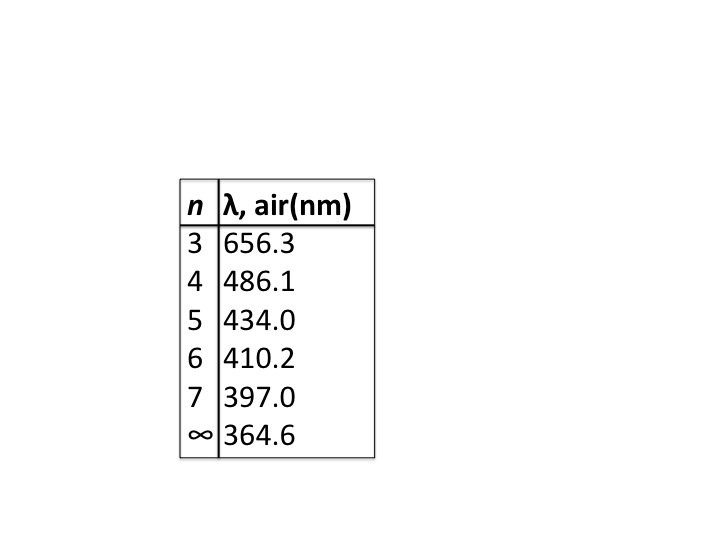
\includegraphics[width=0.4\textwidth]{balmertable} % Include the image placeholder.png
\caption{Table}
\end{center}
\end{figure}


\section{Third hydrogen spectra - Paschen series}
\begin{figure}[h]
\begin{center}
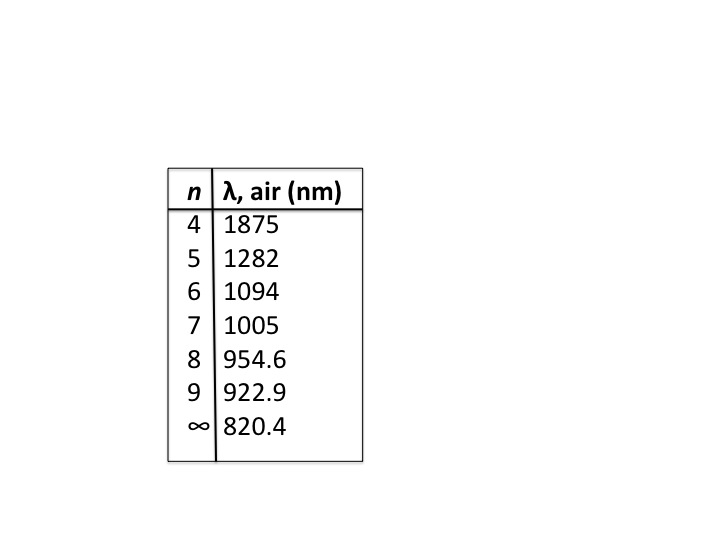
\includegraphics[width=0.4\textwidth]{paschentable} % Include the image placeholder.png
\caption{Table}
\end{center}
\end{figure}

The Paschen lines all lie in the infrared band. It overlaps with the next (Brackett) series, i.e. the shortest line in the Brackett series has a wavelength that falls among the Paschen series. All subsequent series overlap.

\section{Emission and absorption spectra}

The line emission spectra is produced when excited electrons which with values of n greater than 1 fall back to the n=1 ground state, either directly, or by way of intermediate-n states. But if light from a continuous source passes through an atmosphere of hydrogen, those wavelengths that correspond to the allowed transitions are absorbed, and appear as dark lines superimposed on the continuous spectrum.

\begin{figure}[h]
\begin{center}
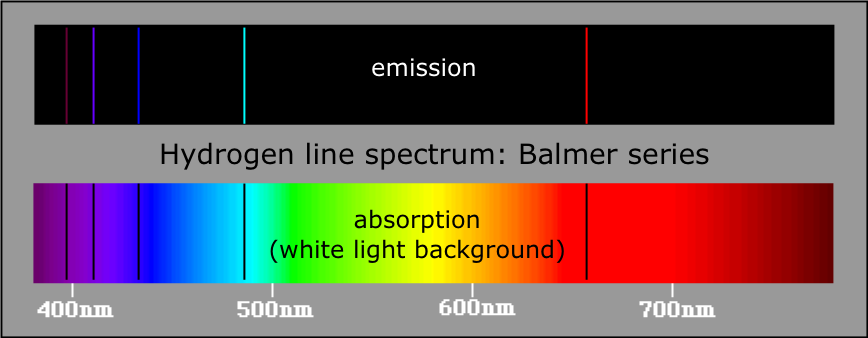
\includegraphics[width=0.4\textwidth]{balmer} % Include the image placeholder.png
\caption{Spectra}
\end{center}
\end{figure}

These dark absorption lines were first observed by William Wollaston in his study of the solar spectrum. In 1814, Joseph von Fraunhofer (1787-1826) re-discovered them and made accurate measurements of 814 lines, including the four most prominent of the Balmer lines.

\section{Bibliography}
The following websites were used:

1)  http://www.chem1.com/acad/webtext/atoms/atpt-3.html

2) http://www.iun.edu/~cpanhd/C101webnotes/modern-atomic-theory/Bohr-model.html

3) https://en.wikipedia.org/wiki/Hydrogen_spectral_series

\end{document}
